\documentclass[border=3pt,tikz]{standalone}
% \usepackage{physics}
\usepackage{tikz}
% \usepackage[outline]{contour} % glow around text
% \contourlength{1.35pt}
\usetikzlibrary{calc}
%\usetikzlibrary{angles,quotes} % for pic
%\usetikzlibrary{arrows.meta}
%\usetikzlibrary{patterns}

\begin{document}


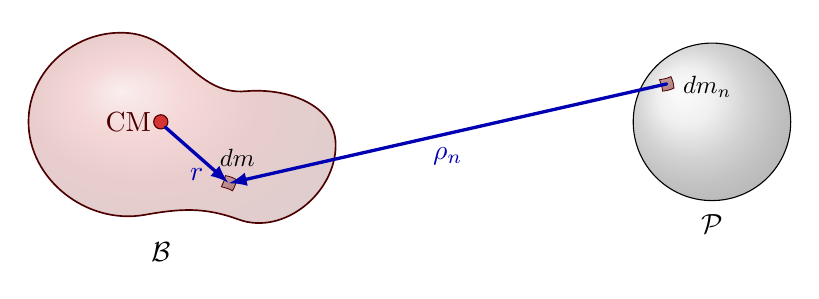
\begin{tikzpicture}[
    >=latex,
    rvec/.style={->,color=blue!70!black,very thick, line cap=round},
    vvec/.style={->,color=green!60!black,very thick,line cap=round},
    CM/.style={color=red!30!black,fill=red!80!black!80},
    mass/.style={line width=0.6,draw=red!30!black,top color=red!40!black!30,bottom color=red!40!black!10,shading angle=30},
    dark mass/.style={line width=0.3,draw=red!30!black,top color=red!40!black!40, bottom color=red!40!black!50,shading angle=30}
    ]
% PARALLEL AXIS (STEINER'S) THEOREM
\def\L{1.2}    % size scale
\def\A{1.8}    % height axis above body
\def\d{1.5}    % distance parallel axis to CM
\def\ang{-20}  % angle connection between axes
\def\anga{72}  % angle axes
\def\bodyshape{
  (-100:1.0*\L) to[out=190,in=-90]
  (180:1.4*\L) to[out=90,in=175]
  (110:1.0*\L) to[out=-5,in=185]
  ($(R)+(110:0.8*\L)$) to[out=5,in=90]
  ($(R)+(15:0.7*\L)$) to[out=-90,in=-20]
  ($(R)+(-120:0.7*\L)$) to[out=160,in=10] cycle
}
\def\body{ % shape
  \fill[ball color=red!80!black] \bodyshape;
  \draw[line width=0.6,draw=red!30!black,fill=red!60!black!5,fill opacity=0.85]
    \bodyshape;
  %\fill[mass] \bodyshape;
}
\def\ys{0.6}     % vertical minor axis ellipse
\def\ri{0.56*\d} % small mass m_i distance from axis
\def\angi{210}   % small mass m_i polar angle
\def\dx{0.15}    % size small mass m_i
\def\massi{
  \draw[dark mass,rotate=\ang+\angi+30] % mass m_i
    (Ri)++(-45:{\dx/sqrt(2)}) to[out=95,in=-100]++
    (90:\dx) to[out=170,in=10]++
    (180:\dx) to[out=-100,in=100]++
    (-90:\dx) to[out=10,in=175]++ (0:\dx) -- cycle;
}
    \def\angi{240}                 % small mass m_i polar angle
    \coordinate (M) at (0,0);      % center of mass
    \node[below=40] at (M) {$\mathcal{B}$};

    \coordinate (R) at (\ang:\d);  % intersection with new axis
    \path[rotate around={\ang:(R)}]
        (R) --++ (\angi:{\ri} and {\ys*\ri}) coordinate(Ri); % small mass m_i

    % BODY
    % \draw (M) --++ (\anga-180:1.5*\L) node[above left] {$I_\text{cm}$}; % axis below
    % \draw (R) --++ (\anga-180:1.1*\L) node[above=4,right=2] {$I$}; % axis below
    \body

    % CENTER OF MASS & MASS i
    \draw[CM] (M) circle(0.09) node[above=0,left] {CM}; % center of mass point
    \massi
    \node[right=3,above=3,scale=0.9] at (Ri) {$dm$};

    % VECTORS
    \draw[rvec] (M)++(-50:0.09) -- ($(M)!0.99!(Ri)$) node[pos=0.5,below=1] {$r$};

    % PRIMARY SPHERE
    \coordinate (P) at ($(M) + (7,0) $);
    \node[below=30] at (P) {$\mathcal{P}$};
    \shade[ball color = gray!40, opacity = 0.4] (P) circle (1cm);
    \draw (P) circle (1cm);
    
    % primary mass element m_n
    % \path (P)
    \coordinate (Mn) at ($ (P) + (140:0.75) $);
    \node[below=1,scale=0.9,right=3] at (Mn) {$d m_n$};

    \draw[dark mass,rotate=195] % mass m_n
        (Mn)++(-45:{\dx/sqrt(2)}) to[out=95,in=-100]++
        (90:\dx) to[out=170,in=10]++
        (180:\dx) to[out=-100,in=100]++
        (-90:\dx) to[out=10,in=175]++ (0:\dx) -- cycle;

    \draw[rvec] (Mn) -- (Ri) node[pos=0.5,below=1] {$\rho_n$};
\end{tikzpicture}
\end{document}
